\documentclass[journal, spanish]{IEEEtran}

% Paquetes necesarios
\usepackage[T1]{fontenc}
\usepackage[utf8]{inputenc}
\usepackage{babel}
\usepackage{cite}
\usepackage{graphicx}
\usepackage{float}
\usepackage{listings}
\usepackage{xcolor}


% Configuración de las cabeceras
\markboth{Estructuras De Datos}{Taller No. 3 Y 4}


% Configuración de las secciones
\title{Taller No. 3 Y 4}
\author{James Andres Cespedes Ibarra\thanks{} \\
\textit{Fundación Universitaria Konrad Lorenz} \\
}

\definecolor{codegreen}{rgb}{0,0.6,0}
\definecolor{codegray}{rgb}{0.5,0.5,0.5}
\definecolor{codepurple}{rgb}{0.58,0,0.82}
\definecolor{backcolour}{rgb}{0.95,0.95,0.92}

\lstdefinestyle{codestyle}{
    backgroundcolor=\color{backcolour},   
    commentstyle=\color{codegreen},
    keywordstyle=\color{magenta},
    numberstyle=\tiny\color{codegray},
    stringstyle=\color{codepurple},
    basicstyle=\ttfamily\footnotesize,
    breakatwhitespace=false,         
    breaklines=true,                 
    captionpos=b,                    
    keepspaces=true,                 
    numbers=left,                    
    numbersep=5pt,                  
    showspaces=false,                
    showstringspaces=false,
    showtabs=false,                  
    tabsize=2
}

\begin{document}

% Creación del título
\maketitle

% Creación del abstract
\begin{abstract}

Analizaremos fragmentos de código mediante notación Big-O con el fin de reforzar habilidades e interpretación de código y su complejidad.

\end{abstract}

% Resultados
\section{Resultados}

Después de realizado el ejercicio de la investigación podemos concluir que mediante el uso de la tecnología y del análisis podemos optimizar nuestros algoritmos con el fin de mejor la eficiencia de los mismos.

\subsection{Algoritmo No. 1}

Como solución a la primera pregunta "Desarrollar un algoritmo que aplique Memorización para mostrar la clasificación de las palabras más repetidas" se propone el siguiente código desarrollado en Python.

\lstset{style=codestyle}
\begin{lstlisting}[language=Python]

from collections import defaultdict

def contar_palabras_largas(texto, longitud_minima=5):
    frecuencias = defaultdict(int)
    palabras = texto.split()

    for palabra in palabras:
        palabra = palabra.lower()

        if len(palabra) >= longitud_minima:
            frecuencias[palabra] += 1

    return frecuencias

def mostrar_palabras_largas_mas_repetidas(texto, num_palabras=10, longitud_minima=5):

    frecuencias = contar_palabras_largas(texto, longitud_minima)

    palabras_ordenadas = sorted(frecuencias.items(), key=lambda x: x[1], reverse=True)

    print(f"Palabras largas más repetidas (longitud >= {longitud_minima}, top {num_palabras}):")
    for palabra, frecuencia in palabras_ordenadas[:num_palabras]:
        print(f"{palabra}: {frecuencia}")

texto = """
    " La programación en Python es clave para el trabajo con datos ",
    " Los programadores en Java tienen un alto interés en pasar a Python ",
    " La optimización de algoritmos es fundamental en el desarrollo de software ",
    " Las bases de datos relacionales son esenciales para muchas aplicaciones ",
    " El paradigma de programación funcional gana popularidad ",
    " La seguridad informática es un tema crucial en el desarrollo de aplicaciones web ",
    " Los lenguajes de programación modernos ofrecen abstracciones poderosas ",
    " La inteligencia artificial está transformando diversas industrias ",
    " El aprendizaje automático es una rama clave de la ciencia de datos ",
    " Las interfaces de usuario intuitivas mejoran la experiencia del usuario ",
    " La calidad del código es esencial para mantener un proyecto exitoso ",
    " La agilidad en el desarrollo de software permite adaptarse a cambios rápidamente ",
    " Las pruebas automatizadas son cruciales para garantizar la estabilidad del software ",
    " La modularización del código facilita la colaboración en equipos de programadores ",
    " El control de versiones es necesario para rastrear cambios en el código ",
    " La documentación clara es fundamental para que otros entiendan el código ",
    " La programación orientada a objetos promueve la reutilización de código ",
    " La resolución de problemas es una habilidad esencial en la programación ",
    " La optimización prematura puede llevar a código complicado y difícil de mantener ",
    " El diseño de interfaces de usuario atractivas mejora la usabilidad de las aplicaciones ",
    " El código limpio es esencial para facilitar el mantenimiento ",
    " Los patrones de diseño son soluciones probadas para problemas comunes ",
    " Las pruebas unitarias garantizan el correcto funcionamiento de las partes del código ",
    " El desarrollo ágil prioriza la entrega continua de valor al cliente ",
    " Los comentarios en el código deben ser claros y útiles ",
    " La recursividad es una técnica poderosa en la programación ",
    " Las bibliotecas de código abierto aceleran el desarrollo de software ",
    " La virtualización permite una mejor utilización de los recursos de hardware ",
    " La seguridad en la programación web es fundamental para prevenir ataques ",
    " Los principios SOLID son fundamentales para el diseño de software robusto ",
    " La arquitectura de microservicios permite escalar componentes individualmente ",
    " La refactorización mejora la calidad del código sin cambiar su comportamiento ",
    " Los sistemas distribuidos presentan desafíos en la sincronización de datos ",
    " El enfoque DevOps une el desarrollo y las operaciones para una entrega eficiente ",
    " Las bases de datos NoSQL son útiles para manejar datos no estructurados ",
    " La agilidad en el desarrollo permite adaptarse a cambios del mercado ",
    " Las buenas prácticas en el control de versiones facilitan la colaboración ",
    " La programación concurrente mejora la eficiencia en sistemas multiusuario ",
    " Los marcos de trabajo MVC separan la lógica de la interfaz de usuario ",
    " La interacción entre aplicaciones se logra a través de APIs ",
    " El machine learning permite a las máquinas aprender de los datos ",
    " La analítica de datos ayuda a tomar decisiones basadas en información ",
    " El diseño responsivo garantiza una experiencia consistente en diferentes dispositivos ",
    " Las pruebas de carga verifican el rendimiento de las aplicaciones ",
    " El enfoque centrado en el usuario mejora la usabilidad de las aplicaciones ",
    " La programación reactiva es útil para manejar flujos de datos asincrónicos ",
    " Los contenedores facilitan la implementación y el despliegue de aplicaciones ",
    " La gestión de dependencias es esencial para administrar las bibliotecas externas ",
    " La integración continua automatiza la verificación de cambios en el código ",
    " El aprendizaje profundo es una rama avanzada del machine learning ",
    " La depuración es una habilidad crucial para encontrar y corregir errores ",
    " La criptografía protege la información sensible en aplicaciones ",
    " El desarrollo full-stack abarca tanto el frontend como el backend ",
    " Las pruebas de seguridad ayudan a identificar vulnerabilidades en el software ",
    " La agilidad cultural es clave para adoptar prácticas ágiles de manera efectiva ",
    " La infraestructura como código permite automatizar la gestión de servidores ",
    " Los patrones arquitectónicos guían la estructura general de una aplicación ",
    " El análisis predictivo utiliza datos históricos para predecir tendencias ",
    " Las interfaces API REST son ampliamente utilizadas para comunicarse con aplicaciones ",
    " El rendimiento de las aplicaciones es esencial para brindar una buena experiencia ",
    " La virtualización de servidores reduce costos y facilita la administración ",
    " La ingeniería de software implica la aplicación de métodos sistemáticos ",
    " El código autodocumentado es claro y fácil de entender para otros programadores ",
    " La integración de sistemas conecta diferentes aplicaciones para trabajar juntas ",
    " Las metodologías ágiles promueven la adaptación y la colaboración continua ",
    " El monitoreo de aplicaciones permite identificar y resolver problemas en tiempo real ",
    " El análisis de datos masivos (big data) abre oportunidades para obtener insights ",
    " El diseño de interfaces de usuario es crucial para la experiencia del usuario ",
    " La seguridad en el desarrollo es un proceso constante de mitigación de riesgos "

mostrar_palabras_largas_mas_repetidas(texto)
\end{lstlisting}

\begin{figure}[H]
  \centering
  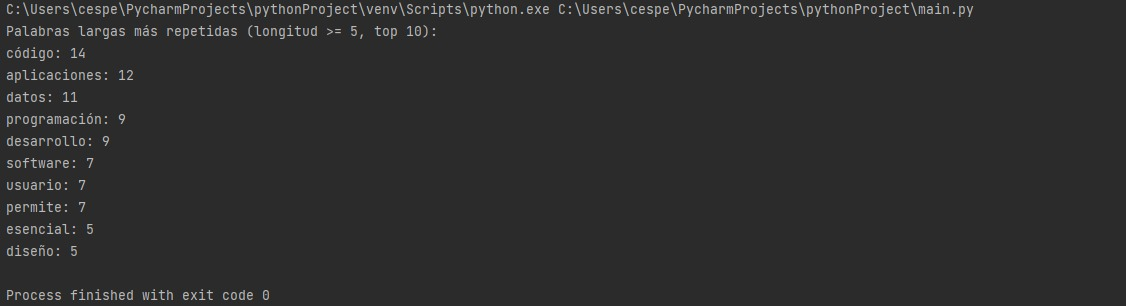
\includegraphics[width=0.5\textwidth]{images/IMG-20230913-WA0001.jpg}
  \caption{Cantidad de repeticiones de palabras dado un texto en el código.}
  \label{fig:nombre_de_tu_imagen}
\end{figure}

La función \textbf{contar palabras largas} toma un texto como entrada y devuelve un diccionario de frecuencias de palabras largas \textbf{(longitud >= 5)} en el texto.

La función divide el texto en palabras utilizando \textbf{texto.split()}. Suponiendo que la longitud promedio de una palabra es \textbf{m} y el número promedio de palabras en el texto es \textbf{k}. Dividir el texto tiene una complejidad de \textbf{O(k * m)}.

Luego, itera sobre cada palabra en el texto y realiza las siguientes operaciones:

Convierte la palabra a minúsculas, lo cual tiene una complejidad de \textbf{O(m)}.
Verifica si la longitud de la palabra es mayor o igual a \textbf{5}, lo cual es una operación \textbf{O(1)}.
Actualiza el contador de frecuencia en el diccionario, que también es una operación \textbf{O(1)} en promedio, ya que se utiliza un diccionario \textbf{defaultdict}.

En resumen, la función \textbf{contar palabras largas} tiene una complejidad temporal total de \textbf{O(k * m)} para dividir el texto en palabras y luego \textbf{O(k * m)} para procesar las palabras y contar las frecuencias. Esto se puede simplificar a \textbf{O(k * m)} en términos asintóticos.

La función \textbf{mostrar palabras largas mas repetidas} toma el resultado del conteo de palabras largas y realiza las siguientes operaciones:

Ordena el diccionario de frecuencias, lo cual tiene una complejidad de \textbf{O(n * log(n))}, donde \textbf{n} es el número de palabras únicas largas en el texto.

Luego, imprime las 10 palabras largas más repetidas, lo cual es una operación \textbf{O(1)} ya que estamos limitando la salida a un número fijo de palabras.

Para este ejemplo, la complejidad temporal total del algoritmo es:

\textbf{O(k * m)} para dividr el texto en palabras .

\textbf{O(m)} para convertirlo a minúsculas.

\textbf{O(1)} para verificar si la longitud de la palabra es mayor o igual a \textbf{5}.

\textbf{O(1)} Actualiza el contador de frecuencia en el diccionario

\textbf{O(n * log(n))} para ordenar el diccionario de frecuencias.

\textbf{O(1)} para imprimir las 10 palabras largas más repetidas.

Por lo tanto, la complejidad general del algoritmo es \textbf{O(n) + O(m) + O(k * m) + O(k)}, dando como resultado \textbf{O(n * m)}.

Por lo tanto, la complejidad general del algoritmo es \textbf{O(k * m)} + \textbf{O(m)} + \textbf{O(1)} + \textbf{O(1)} + \textbf{O(n * log(n))} + \textbf{O(1)}, dando como resultado \textbf{O(n * log(n))}.

\subsection{Algoritmo No. 2}

Como solución a la primera pregunta "Desarrollar un algoritmo que aplique Memorización para mostrar la clasificación de las palabras más repetidas" se propone el siguiente código desarrollado en Python.

\lstset{style=codestyle}
\begin{lstlisting}[language=Python]
    
    documento = [
    "La programación en Python es clave para el trabajo con datos",
    "Los programadores en Java tienen un alto interés en pasar a Python",
    "La optimización de algoritmos es fundamental en el desarrollo de software",
    "Las bases de datos relacionales son esenciales para muchas aplicaciones",
    "El paradigma de programación funcional gana popularidad",
    "La seguridad informática es un tema crucial en el desarrollo de aplicaciones web",
    "Los lenguajes de programación modernos ofrecen abstracciones poderosas",
    "La inteligencia artificial está transformando diversas industrias",
    "El aprendizaje automático es una rama clave de la ciencia de datos",
    "Las interfaces de usuario intuitivas mejoran la experiencia del usuario",
    "La calidad del código es esencial para mantener un proyecto exitoso",
    "La agilidad en el desarrollo de software permite adaptarse a cambios rápidamente",
    "Las pruebas automatizadas son cruciales para garantizar la estabilidad del software",
    "La modularización del código facilita la colaboración en equipos de programadores",
    "El control de versiones es necesario para rastrear cambios en el código",
    "La documentación clara es fundamental para que otros entiendan el código",
    "La programación orientada a objetos promueve la reutilización de código",
    "La resolución de problemas es una habilidad esencial en la programación",
    "La optimización prematura puede llevar a código complicado y difícil de mantener",
    "El diseño de interfaces de usuario atractivas mejora la usabilidad de las aplicaciones",
    "El código limpio es esencial para facilitar el mantenimiento",
    "Los patrones de diseño son soluciones probadas para problemas comunes",
    "Las pruebas unitarias garantizan el correcto funcionamiento de las partes del código",
    "El desarrollo ágil prioriza la entrega continua de valor al cliente",
    "Los comentarios en el código deben ser claros y útiles",
    "La recursividad es una técnica poderosa en la programación",
    "Las bibliotecas de código abierto aceleran el desarrollo de software",
    "La virtualización permite una mejor utilización de los recursos de hardware",
    "La seguridad en la programación web es fundamental para prevenir ataques",
    "Los principios SOLID son fundamentales para el diseño de software robusto",
    "La arquitectura de microservicios permite escalar componentes individualmente",
    "La refactorización mejora la calidad del código sin cambiar su comportamiento",
    "Los sistemas distribuidos presentan desafíos en la sincronización de datos",
    "El enfoque DevOps une el desarrollo y las operaciones para una entrega eficiente",
    "Las bases de datos NoSQL son útiles para manejar datos no estructurados",
    "La agilidad en el desarrollo permite adaptarse a cambios del mercado",
    "Las buenas prácticas en el control de versiones facilitan la colaboración",
    "La programación concurrente mejora la eficiencia en sistemas multiusuario",
    "Los marcos de trabajo MVC separan la lógica de la interfaz de usuario",
    "La interacción entre aplicaciones se logra a través de APIs",
    "El machine learning permite a las máquinas aprender de los datos",
    "La analítica de datos ayuda a tomar decisiones basadas en información",
    "El diseño responsivo garantiza una experiencia consistente en diferentes dispositivos",
    "Las pruebas de carga verifican el rendimiento de las aplicaciones",
    "El enfoque centrado en el usuario mejora la usabilidad de las aplicaciones",
    "La programación reactiva es útil para manejar flujos de datos asincrónicos",
    "Los contenedores facilitan la implementación y el despliegue de aplicaciones",
    "La gestión de dependencias es esencial para administrar las bibliotecas externas",
    "La integración continua automatiza la verificación de cambios en el código",
    "El aprendizaje profundo es una rama avanzada del machine learning",
    "La depuración es una habilidad crucial para encontrar y corregir errores",
    "La criptografía protege la información sensible en aplicaciones",
    "El desarrollo full-stack abarca tanto el frontend como el backend",
    "Las pruebas de seguridad ayudan a identificar vulnerabilidades en el software",
    "La agilidad cultural es clave para adoptar prácticas ágiles de manera efectiva",
    "La infraestructura como código permite automatizar la gestión de servidores",
    "Los patrones arquitectónicos guían la estructura general de una aplicación",
    "El análisis predictivo utiliza datos históricos para predecir tendencias",
    "Las interfaces API REST son ampliamente utilizadas para comunicarse con aplicaciones",
    "El rendimiento de las aplicaciones es esencial para brindar una buena experiencia",
    "La virtualización de servidores reduce costos y facilita la administración",
    "La ingeniería de software implica la aplicación de métodos sistemáticos",
    "El código autodocumentado es claro y fácil de entender para otros programadores",
    "La integración de sistemas conecta diferentes aplicaciones para trabajar juntas",
    "Las metodologías ágiles promueven la adaptación y la colaboración continua",
    "El monitoreo de aplicaciones permite identificar y resolver problemas en tiempo real",
    "El análisis de datos masivos (big data) abre oportunidades para obtener insights",
    "El diseño de interfaces de usuario es crucial para la experiencia del usuario",
    "La seguridad en el desarrollo es un proceso constante de mitigación de riesgos"
]

def buscar_documentos(palabra_busqueda, lista_documentos):

    documentos_coincidentes = []

    for indice, documento in enumerate(lista_documentos):

        documento = documento.lower()

        palabras = documento.split()

        if palabra_busqueda.lower() in palabras:

            documentos_coincidentes.append((indice, documento))

    return documentos_coincidentes

palabra_a_buscar = "documento"

documentos_coincidentes = buscar_documentos(palabra_a_buscar, documento)

if len(documentos_coincidentes) > 0:
    print(f"Documentos que contienen la palabra '{palabra_a_buscar}':")
    for indice, documento in documentos_coincidentes:
        print(f"Documento {indice + 1}: {documento}")
else:
    print(f"No se encontraron documentos que contengan la palabra '{palabra_a_buscar}'.")
\end{lstlisting}

\begin{figure}[H]
  \centering
  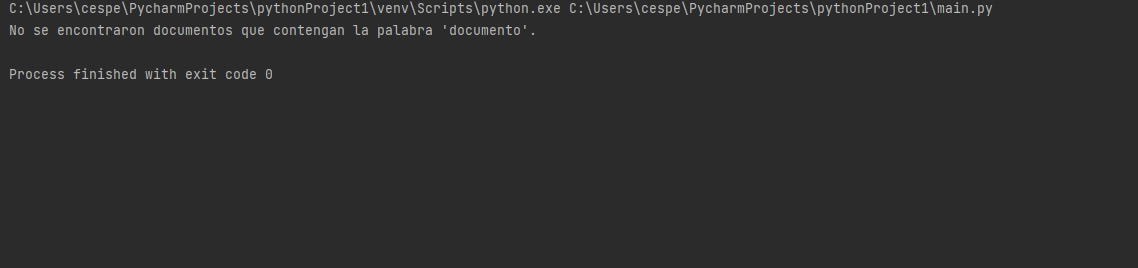
\includegraphics[width=0.5\textwidth]{images/IMG-20230913-WA0002.jpg}
  \caption{Cantidad de repeticiones de palabras dado un texto en el código.}
  \label{fig:nombre_de_tu_imagen}
\end{figure}

La lista \textbf{documento} contiene un total de \textbf{n} documentos.

La función \textbf{buscar documentos} recorre cada documento en la lista \textbf{documento}. Por lo tanto, tiene una complejidad temporal de \textbf{O(n)}.

Para cada \textbf{documento}, se realiza lo siguiente:

El documento se convierte a minúsculas, lo cual tiene una complejidad de \textbf{O(m)}, donde \textbf{m} es la longitud del documento.

Luego, el documento se divide en palabras utilizando \textbf{documento.split()}. 

Suponiendo que la longitud promedio de un documento es \textbf{m}, y el número promedio de palabras en un documento es \textbf{k}. Entonces, dividir el documento tiene una complejidad de \textbf{O(k * m)}.

Después de dividir el documento, se verifica si la palabra clave está presente en las palabras del documento.

Esto tiene una complejidad de \textbf{O(k)}, donde \textbf{k} es el número de palabras en el documento.

Si el documento contiene la palabra clave, se agrega a la lista \textbf{documentos coincidentes}.

Esto es una operación \textbf{O(1)} amortizada, ya que agregar a una lista generalmente tiene un costo constante en Python.

Para este ejemplo, la complejidad temporal total del algoritmo es:

\textbf{O(n)} para recorrer todos los documentos.

Para cada documento:

\textbf{O(m)} para convertirlo a minúsculas.

\textbf{O(k * m)} para dividir el documento en palabras.

\textbf{O(k)} para verificar si contiene la palabra clave.

Por lo tanto, la complejidad general del algoritmo es \textbf{O(n) + O(m) + O(k * m) + O(k)}, dando como resultado \textbf{O(n * m)}.

% Conclusiones
\section{Conclusiones}
Después de realizado el ejercicio podemos concluir que mediante el uso de la tecnología y el análisis de los datos obtenidos podemos optimizar nuestros algoritmos en pro de realizar un eficiente consumo de los mismos en nuestras máquinas o servidores.

% Bibliografía
\bibliographystyle{IEEEtran}

\cite{assailly2017road}
\cite{johnsson2018search}
\cite{wegman2017future}

\bibliography{bibliography}
\vspace{12pt}
\end{document}

